The benchmark is built to answer a specific falsification question:
\emph{can a scalar controller class explain low-regret prefix actions, or do we need a richer \processstate view?}

\paragraph{Exact-checker domains.}
The arithmetic and linear-equations domains admit exact or near-exact prefix evaluation under rollout.
This makes it possible to compute oracle utilities for \continue, \revise, and \abstain at intermediate states.
The key advantage over final-answer evaluation is that we can reason about intervention timing, not only end-task success.
The benchmark samples decision points along base traces generated by a fixed reasoner, and augments them with recoverable perturbations when needed to cover revise-relevant states.
The \revise action is deliberately bounded: it rolls back one local step and then resumes rollout from the repaired prefix.
This keeps the action space simple enough for oracle evaluation while still exposing meaningful timing decisions.

\paragraph{Determinacy and crossing.}
Two benchmark quantities matter most.
The oracle determinacy rate measures how often the best action is meaningfully separated from the next-best action.
Crossing mass measures how often nearby scalar scores correspond to different optimal actions.
If crossing mass is large only in low-determinacy regions, the phenomenon could be dismissed as noise.
If it persists in high-determinacy regions, ordered scalar thresholding becomes a poor model of the control problem.

\begin{table}[t]
\centering
\caption{Oracle benchmark diagnostics for the two exact-checker domains. ``Determinacy'' is the fraction of prefixes whose top action is clearly separated from the runner-up; ``Crossing'' is the fraction of scalar-score neighborhoods that still contain different oracle-optimal actions. The main point is not only that crossing exists, but that it persists after filtering to high-determinacy prefixes.}
\label{tab:benchmark}
\begin{tabular}{lrrrrr}
\toprule
Domain & Prefixes & Determinacy & Crossing & High-det crossing & Mean gap \\
\midrule
Linear equations & 58 & 0.741 & 0.741 & 0.767 & 0.492 \\
Arithmetic & 62 & 0.855 & 0.806 & 0.793 & 0.663 \\
\bottomrule
\end{tabular}
\end{table}

Table~\ref{tab:benchmark} summarizes the benchmark.
Both domains show substantial high-determinacy crossing, which is the main mechanism-level reason to reject a simple scalar-ordering view.
The result is especially important because the two domains do \emph{not} agree on the strongest downstream controller ranking.
That asymmetry is informative: it shows that the benchmark is identifying a control problem, not simply selecting one fixed best controller.

\begin{figure}[t]
\centering
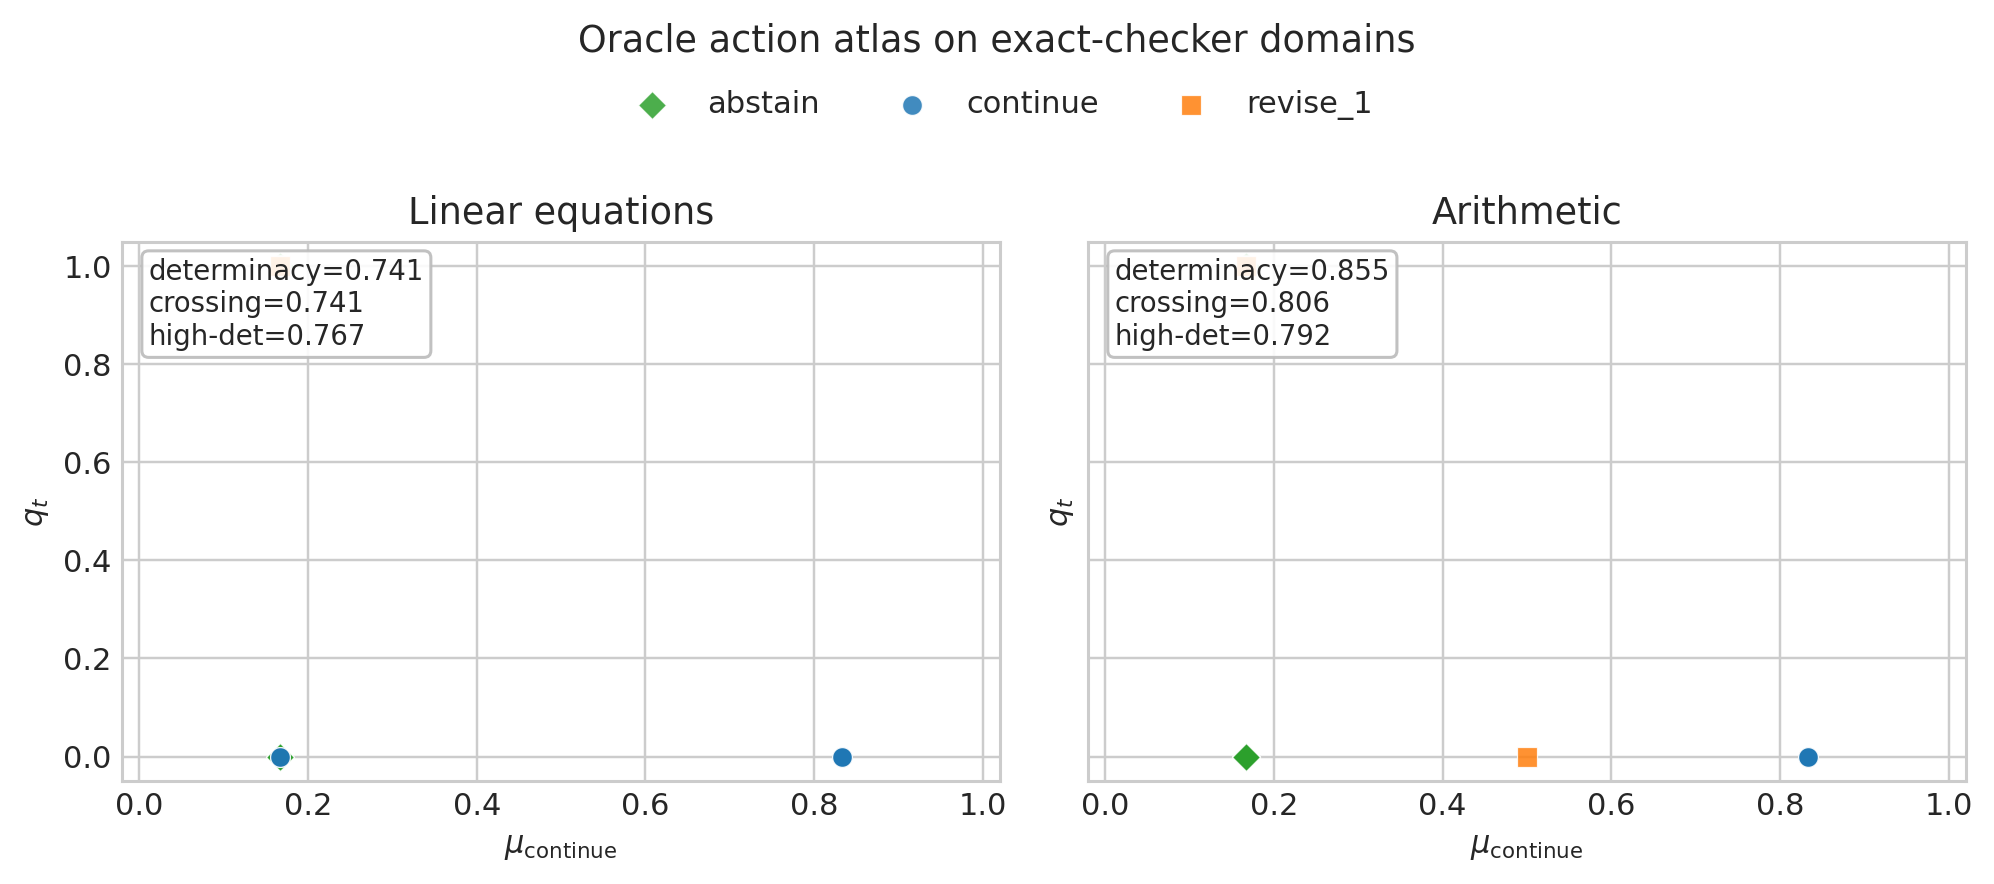
\includegraphics[width=\linewidth]{figures/benchmark_atlas.pdf}
\caption{Oracle action atlas on the two exact-checker domains. Each point is a sampled prefix, placed by continuation score $\mu_{\continue}$ and local invalidity estimate $q_t$, and colored by the oracle-optimal action among \continue, \revise, and \abstain. The visual takeaway is that nearby scalar locations still map to different actions in both domains, which is exactly the crossing phenomenon the benchmark is designed to expose.}
\label{fig:atlas}
\end{figure}

Figure~\ref{fig:atlas} is the corresponding visual summary.
It makes the core benchmark point visual:
nearby scalar scores do not imply nearby optimal actions, and that effect survives determinacy filtering.

These diagnostics support the strongest benchmark claim in the paper.
We do not need to prove that \emph{every} one-dimensional encoding fails.
We need only show that simple continuation-score thresholding, and more generally a single ordered confidence score, is not a sufficient account of low-regret prefix control.
The benchmark does that.
